\chapter{Docking Molecolare}
\textit{Questo capitolo tratta dell'idea che ha ispirato questa tesi, ossia gli effetti negativi dei pesticidi sulle api da miele e del processo che ha portato allo sviluppo del software realizzato che visualizza come le molecole di specifici pesticidi si dispongono, in maniera spaziale, quando sono legate ai recettori delle api, questo processo viene definito docking molecolare e successivamente il software estrae i legami che si vengono a formare.}

\vskip 1cm

\section{I pesticidi e gli insetti impollinatori}
Le api recano importanti benefici e servizi ecologici per la società. Con l’impollinazione le api svolgono una funzione strategica per la conservazione della flora, contribuendo al miglioramento ed al mantenimento della biodiversità.\newline
In botanica, l’impollinazione è quel processo che consiste nel trasporto dei pollini dalla parte maschile e quella femminile dell’apparato riproduttivo delle piante. Grazie ad agenti atmosferici e sopratutto al lavoro incessante degli insetti impollinatori, soprattutto le api, il polline viene trasportato da una pianta all’altra rendendo possibile la fecondazione di un organismo vegetale della stessa specie e la conseguente produzione di semi e frutti. Una diminuzione delle api può quindi rappresentare una importante minaccia per gli ecosistemi naturali in cui esse vivono. L’agricoltura, d’altro canto, ha un enorme interesse a mantenere le api quali efficaci agenti impollinatori. La Food and Agriculture Organization - FAO ha informato la comunità internazionale dell’allarmante riduzione a livello mondiale di insetti impollinatori, tra cui \textit{Apis mellifera}, le api da miele. Circa l’84\% delle specie di piante e l’80\% della produzione alimentare in Europa dipendono in larga misura dall’impollinazione ad opera delle api ed altri insetti pronubi\cite{bellucciapi}. Pertanto, il valore economico del servizio di impollinazione offerto dalle api risulta fino a dieci volte maggiore rispetto al valore del miele prodotto.\newline 
Da un rapporto dell’Unione Internazionale per la Conservazione della Natura (LUCN) risulta che il 10\% delle specie selvatiche di api (\textit{Apis mellifera}) sarebbe in via di estinzione e un altro 5\% sarebbe a rischio. Una delle principali cause sono i pesticidi, i quali influenzano l’apprendimento, la capacità riproduttiva, i comportamenti sociali di questi insetti e l'orientamento. \newline
La mortalità delle api del miele (\textit{Apis mellifera}) è un fenomeno che si acuisce soprattutto in primavera e che rischia di compromettere la fondamentale funzione ecologica di questi insetti impollinatori per l’intero ecosistema.\newline
Un’indagine di campo del Centro di referenza nazionale per l’apicoltura dell’Istituto Zooprofilattico Sperimentale delle Venezie nell’ambito di alcune morie riscontrate ha rilevato la presenza, in campioni di api morte, di residui di pesticidi e di alcuni virus delle api. Le infezioni virali potrebbero peggiorare l’impatto già negativo dei pesticidi sulla salute delle api, mettendo ulteriormente in pericolo la sopravvivenza delle colonie.\newline
Lo studio è stato effettuato su 94 campioni, provenienti dal Nord-est dell’Italia e raccolti durante la primavera 2014, prendendo in considerazione 150 principi attivi e 3 virus delle api. Lo studio è pubblicato su Journal of Apicultural Research. I ricercatori hanno riscontrato la presenza di almeno un principio attivo nel 72,2\% dei campioni (api morte). Gli insetticidi sono i più abbondanti (59,4\%), principalmente quelli appartenenti alla classe dei neonicotinoidi (41,8\%), seguiti da fungicidi (40,6\%) e acaricidi (24,1\%). Gli insetticidi più frequentemente rilevati sono rappresentati da imidacloprid, chlorpyrifos, tau-fluvalinate e cyprodinil.\newline
La presenza di una possibile relazione tra la mortalità primaverile delle api e l’impiego di trattamenti antiparassitari in agricoltura potrebbe contribuire a comprendere meglio fenomeni complessi come la moria delle api e lo spopolamento degli alveari, che negli ultimi dieci anni hanno colpito questo settore\cite{martinello2017spring}.\newline
Poichè i pesticidi vengono impiegati lontano dagli alveari e dalle zone loro circostanti, diventa importante comprendere quali sono gli effetti dei pesticidi a concentrazioni sub-letali e come questi possono in qualche modo alterare i parametri vitali descritti precedentemente. Sono iniziati quindi studi di predizione usando docking molecolare, che cercano di mettere in relazione le interazioni tra le proteine di api e le molecole di pesticidi con effetti a livello metabolico che possono giustificare l’incremento di mortalità. Partendo da questi studi, lo scopo della presente tesi è stato quello di progettare un software capace di automatizzare i processi di preparazione degli input per l’analisi di docking molecolare, che includono la ricerca nei database online e il download delle strutture 3D delle molecole di ligando (pesticida) e di recettori (proteine). Inoltre, il software è in grado di eseguire l’analisi di docking molecolare richiamando e interagendo con software specializzati per il docking, come Autodock Vina e, soprattutto, di presentare in maniera semplice ed interpretabile l’analisi dei risultati della predizione dell’interazione proteina/ligando.\newline

\begin{figure}[H]
    \centering
    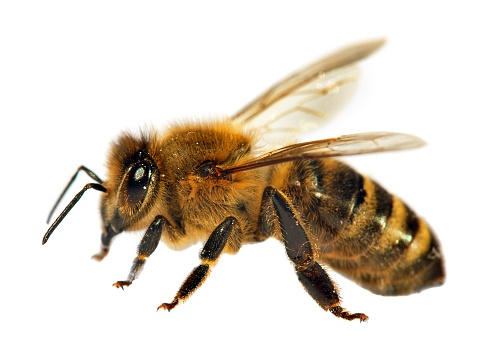
\includegraphics{immagini/capitolo1/apisMellifera.png}
    \caption{Esemplare adulto di Apis Mellifera}
    \label{fig:Apis Mellifera}
\end{figure}

\section{Cos'è il Docking Molecolare}
Il \textbf{docking molecolare} è una tecnica computazionale che permette lo studio dell’interazione tra due molecole. Viene utilizzata, in particolare, per studiare l’interazione delle proteine con altre molecole di interesse biomedico quali acidi nucleici, farmaci, e altre proteine. Il docking si interessa del modo in cui le molecole si agganciano l’una all’altra.\newline
Per effettuare il docking tra due molecole occorre conoscerne la struttura tridimensionale: questa può essere ottenuta per via sperimentale tramite cristallografia a raggi X o per risonanza magnetica nucleare (NMR, Nuclear magnetic resonance), oppure può essere costruita teoricamente. Per studiare il docking è necessario modellizzare le interazioni fondamentali tra i costituenti atomici delle molecole. Queste interazioni sono approssimate in modo adeguato da potenziali di interazione classici (interazioni elettrostatiche, di volume escluso, nonché intramolecolari). Tali potenziali sono utilizzati anche per studiare l’evoluzione temporale delle molecole.\newline 
Il docking è possibile grazie alla potenza di calcolo dei computer moderni e allo sviluppo di adeguati algoritmi. Per poter studiare efficacemente le interazioni strutturali tra molecole (in particolare tra proteine e ligandi) si fa anche ricorso a un’analisi statistica: si utilizzano cioè le strutture di proteine e ligandi note sperimentalmente e che possono essere usate come modello (\textit{template}). A questo fine è stato necessario, in anni recenti, sviluppare grandi database (per es., la RCSB Protein Data Bank (RCSB-PDB)) e algoritmi e talvolta linguaggi di programmazione adatti per la ricerca rapida nei database. Nell’ambito delle bioscienze, le proteine sono di gran lunga le molecole più studiate, per l’importanza che ricoprono nei processi biologici. L’interazione tra proteine è però estremamente complessa in quanto sono oggetti flessibili, ossia in grado di assumere nel tempo, grazie alle fluttuazioni termiche, un insieme molto vasto di conformazioni: è proprio questa flessibilità che permette alle proteine di interagire efficacemente tra loro. Dal punto di vista computazionale è tuttavia difficile tenere conto efficacemente del panorama conformazionale. Le tecniche che simulano la dinamica possono infatti accedere a tempi di scala ancora limitati (nanosecondi) e le tecniche di docking fanno riferimento a strutture cristallografiche fisse che sono ottenute in condizioni sperimentali lontane dall’ambiente funzionale. Le strutture NMR hanno il vantaggio di essere ottenute quasi in \textit{vivo} (ossia con minore impatto della sperimentazione sulla struttura proteica), ma sono difficili da ottenere e hanno risoluzione spaziale inferiore.\newline
Nonostante le difficoltà, il docking è estremamente utile per lo studio dell’interazione tra proteine e piccoli ligandi. Esistono apposite tecniche di drug design in cui si progetta una molecola in funzione della struttura cui si dovrà legare per espletare la funzione voluta. Nel considerare la configurazione ottimale del legame tra proteina e ligando, vanno inoltre considerati non solo i caratteri topologici di complementarietà (del tipo chiave-serratura), ma anche il bilancio energetico della configurazione. Questo andrà ottimizzato ricercando lo stato in cui l’energia libera del sistema proteina-ligando sia minima, rendendo il loro legame più probabile, e quindi maggiormente stabile rispetto ad altre configurazioni. Poiché esiste un gran numero di configurazioni possibili nelle interazioni tra molecole, sono stati lanciati numerosi progetti di calcolo distribuito con collaborazioni internazionali per fare uno screening su larga scala delle molecole in grado di interagire con specifiche proteine di interesse biomedico come, per es., quelle legate al virus HIV o all’infezione malarica. Si pensa in questo modo di riuscire a ottimizzare l’efficacia dei farmaci esistenti, nonché a scoprirne di nuovi, diretti verso specifici bersagli terapeutici molecolari\cite{dockingMolecolare}.\newline
Gli algoritmi di docking sono formati da due componenti fondamentali:

\begin{itemize}
    \item L’algoritmo di ricerca o \textit{“search algorithm”}
    \item La \textit{“scoring function”}.
\end{itemize} 

Il primo si occupa di generare un insieme di 12 conformazioni del ligando all’interno del sito designato del target, mentre la seconda valuta le \textit{poses} generate, assegnando a ciascuna di esse un punteggio detto \textit{“score”} in base a parametri di tipo geometrico ed energetico. Le migliori conformazioni in uscita da questa valutazione sono passate nuovamente all’algoritmo di ricerca, che andrà a creare una nuova generazione di conformazioni partendo dalle migliori soluzioni dell'esecuzione precedente. Il funzionamento iterativo del \textit{search algorithm} e della \textit{scoring function} permettono di ottenere, alla fine di un determinato numero di cicli, un insieme di \textit{poses} che vengono fornite come output all’utente e che sono ritenute essere le migliori soluzioni per il \textit{binding} delle molecole in esame da parte del programma di docking utilizzato.\newline
In generale, il docking molecolare è eseguibile in tre differenti condizioni, che si differenziano l’una dall’altra per i gradi di libertà tenuti in considerazione dall’algoritmo durante il calcolo: 

\begin{enumerate}[label=\Roman{*}., ref=(\Roman{*})]
    \item \textbf{docking a corpo rigido}, che approssima sia il ligando che la proteina come strutture rigide
    \item \textbf{docking semi-flessibile}, che considera il target come rigido, tendendo però in considerazione i gradi di libertà conformazionale del ligando
    \item \textbf{docking flessibile}, in cui vengono considerati i gradi di libertà sia del ligando che dei residui del target nel sito attivo.
\end{enumerate}

Intuitivamente, passando da un approccio a corpo rigido fino ad uno flessibile, la complessità di calcolo aumenta, e proporzionalmente, anche il tempo di esecuzione.\newline
Ad oggi sono disponibili diversi protocolli di docking ognuno dei quali sfrutta una particolare coppia algoritmo di \textit{ricerca-scoring function}.\newline
Il docking molecolare consiste in tre obiettivi principali collegati tra loro: 

\begin{enumerate}[label=\arabic{*}., ref=(\arabic{*})]
    \item predizione della posa
    \item screening virtuale
    \item stima dell'affinità di legame.
\end{enumerate}

Una metodologia di docking di successo deve essere in grado di prevedere correttamente la posa nativa del ligando all'interno del sito di legame del recettore, cioè trovare la geometria sperimentale del ligando entro un certo limite di tolleranza, e le interazioni fisico-chimiche molecolari associate.\newline
Quando si analizzano librerie di composti di grandi dimensioni, il metodo deve essere in grado di distinguere con successo le molecole che si legano da quelle che non si legano e di classificare correttamente questi ligandi tra i migliori composti del database.\newline
Un algoritmo di ricerca e una funzione di score energetico sono gli strumenti di base di una metodologia di docking per generare e valutare le conformazioni dei ligandi. La capacità di gestire con successo la flessibilità molecolare intrinseca di un sistema e di descrivere correttamente l'energia delle interazioni recettore-ligando è cruciale per lo sviluppo di metodologie di docking predittivo che sono utili negli studi prospettici di progettazione di farmaci\cite{guedes2014receptor}.

\begin{figure}[H]
    \centering
    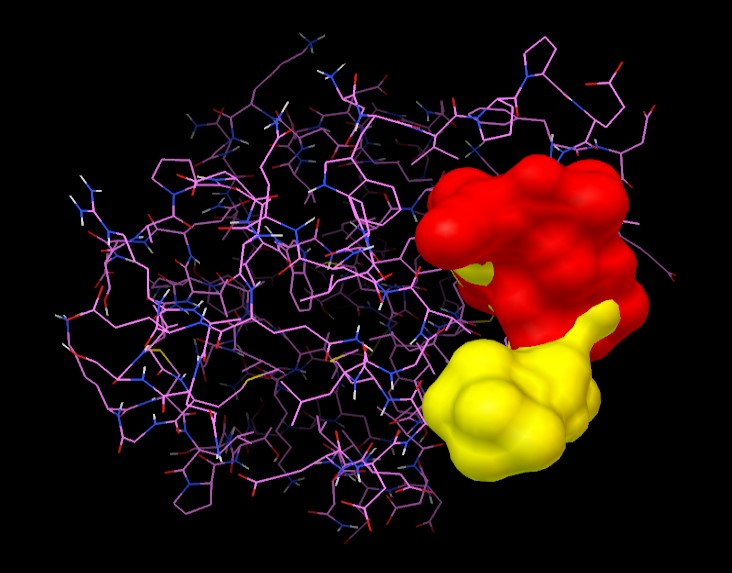
\includegraphics{immagini/capitolo1/dockingMolecolare.png}
    \caption{Rappresentazione del docking tra il ligando acrinathrin e la proteina 2h8v}
    \label{fig:docking molecolare}
\end{figure}

\section{Simulazione}
La \textbf{simulazione} di un processo di docking è un processo molto più che complicato. In tale approccio, la proteina e il ligando sono separati fisicamente da una certa distanza, e il ligando trova la sua posizione nel sito attivo della proteina dopo aver compiuto diversi movimenti nello spazio. Tali movimenti includono rotazioni, traslazioni e torsione di alcuni angoli di rotazione degli atomi. Ognuno di questi movimenti ha un determinato costo energetico nel sistema, dato che dopo ogni mossa viene ricalcolata l'energia totale. Questo approccio rappresenta molto bene quello che accade nella realtà. Di contro, il costo richiesto in termini di tempo e prestazioni è molto elevato.
    
\section{Software per il Docking Molecolare}
I programmi di docking molecolare eseguono un algoritmo di ricerca in cui la conformazione del ligando viene valutata ricorsivamente fino a raggiungere la convergenza all'energia minima. Infine, una funzione di punteggio di affinità, $\Delta$G (Energia potenziale totale in kcal/mol), viene impiegata per classificare le pose candidate come la somma delle energie elettrostatiche e di van der Waals. Le forze trainanti per queste specifiche interazioni nei sistemi biologici mirano alla complementarità tra la forma e l'elettrostatica delle superfici del sito di legame e del ligando o del substrato. \newline
Negli ultimi vent'anni, sono stati sviluppati più di 60 diversi strumenti e programmi di docking sia per uso accademico e commerciali, come DOCK (Venkatachalam et al. 2003), AutoDock (Österberg et al. 2002), FlexX (Rarey et al. 1996), Surflex (Jain 2003), GOLD (Jones et al. 1997), ICM (Schapira et al. 2003), Glide (Friesner et al. 2004), Cdocker, LigandFit (Venkatachalam et al. 2003), MCDock, FRED (McGann et al. 2003), MOE-Dock (Corbeil et al. 2012), LeDock (Zhao e Caflisch 2013), AutoDock Vina (Trott e Olson 2010), rDock (Ruiz-Carmona et al. 2014), UCSF Dock (Allen et al. 2015) e molti altri. \newline 
Tra questi programmi, AutoDock Vina, GOLD e MOE-Dock hanno predetto le pose migliori con gli score migliori. AutoDock e LeDock sono stati in grado di identificare i corretti legami dei ligandi nelle pose. Sia Glide (XP) che AutoDock hanno previsto le pose con un'accuratezza del 90,0\% (Wang et al. 2016). È stato dimostrato che AutoDock ha prodotto fattori di arricchimento più rispetto a Glide in uno studio di screening virtuale contro il Fattore Xa, mentre Glide ha superato AutoDock contro lo stesso bersaglio in un analogo studio di screening virtuale. Nel complesso, è stato riportato recentemente che questi programmi di docking sono in grado di predire pose sperimentali con deviazioni al quadrato della radice (RMSD) in media (RMSD) in media da 1,5 a 2 Å\cite{pagadala2017software}.\newline 
Come mostrato nella Figura 1.3, il software di docking molecolare può aiutarci a individuare la conformazione e l'orientamento ottimali in base alla complementarità e alla pre-organizzazione con un algoritmo specifico, quindi ad applicare una funzione di scoring per prevedere l'affinità del legame e ad analizzare la modalità interattiva\cite{fan2019progress}.

\begin{figure}[H]
    \centering
    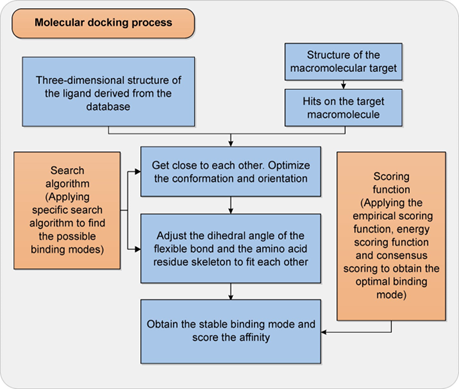
\includegraphics{immagini/capitolo1/processoDockingMolecolare.png}
    \caption{Processo del docking molecolare}
    \label{fig:processo del docking Molecolare}
\end{figure}

\section{Gestione del lavoro}
Il software trattato è frutto del lavoro congiunto del sottoscritto e del mio collega di studi Massimiliano Giordano Orsini con il coordinamento del dottor Ferdinando Febbraio, ricercatore presso l’Istituto di Biochimica e Biologia Cellulare del Consiglio Nazionale delle Ricerche (IBBC-CNR), e mio correlatore di tesi. Il lavoro può essere equiparato ad un vero e proprio progetto software, e si è sviluppato in più fasi. In una prima fase attraverso continue discussioni nell’ambito della biologia ed esempi di utilizzo dei software e delle rispettive analisi, sono stati chiariti una serie di concetti poco familiari a me ed al mio collega. A questa fase sono seguite varie fasi di analisi e di progettazione, per poi passare alla fase di sviluppo, corrispondente alla fase di effettiva implementazione del software. Infine sono state effettuate le fasi di testing funzionale (FAT) e utente (UAT) per individuare e risolvere errori e bug ed approvare il software realizzato. Le varie fasi di sviluppo software non si sono succedute in maniera sequenziale, seguendo quindi i dettami del modello di sviluppo waterfall, bensì le varie fasi sono state inframmezzate l’una con l’altra e, più che come passi di un processo sono state iterazioni cicliche delle stesse, rispettando i paradigmi dello sviluppo agile. Questo processo di sviluppo è stato dettato dalla natura stessa del progetto, poiché a seguito del raggiungimento di un obiettivo, sono state valutate e decise ulteriori implementazioni per dotare di maggiore complementarietà il software prodotto.

\section{Idea e sviluppo}
L’idea nasce dall’attività di tirocinio svolta presso l’IBBC-CNR di Napoli, per un totale di 300 ore, sotto la supervisione del Responsabile del laboratorio di informatica dell’università Parthenope, professor Angelo Ciaramella e del dottor Ferdinando Febbraio dell’IBBC-CNR di Napoli. Il lavoro effettuato è consistito nella realizzazione di un software, del tutto preliminare al progetto di tesi proposto. Lo sviluppo è avvenuto attraverso diverse fasi nelle quali sono stati utilizzati ed implementati i seguenti tools: 

\begin{itemize}
    \item software per l'esecuzione del docking
    \item funzioni di bioinformatica per la preparazione degli input necessari
    \item software per l'analisi dei risultati dell'intero processo.
\end{itemize}

Sono state determinate le componenti software ideali per automatizzare il processo di docking conseguendo risultati efficienti per quanto riguarda l'output e l'analisi dello stesso, offrendo una buona usabilità del prodotto realizzato mediante una semplice ed intuitiva interfaccia grafica.

\section{Descrizione dell'applicazione}
Il progetto di tesi proposto ha come focus principale la realizzazione di un applicativo che effettua il docking tra i ligandi contenuti in specifici pesticidi e i recettori dell’ \textit{Apis mellifera} e l’estrazione dei legami che si vengono a 
formare.\newline
Il nome scelto per l'applicazione realizzata è \textbf{AUtomated DOcking 4 RIsk ASsessment} (\textbf{AUDO4RIAS}) in quanto prova della digitalizzazione della disciplina biologica.\newline
L’applicazione può essere scaricata con le configurazioni di default, direttamente dalla repository di github. Il software realizzato può essere utilizzato in due modalità: 

\begin{itemize}
    \item mediante \textbf{script python da terminale}
    \item mediante \textbf{interfaccia grafica} realizzata seguendo il paradigma model ViewController.
\end{itemize} 

La GUI usufruirà degli stessi script lanciati da riga di comando garantendo le stesse funzionalità secondo i dettami della OOP, ossia riutilizzo del codice funzionante anziché modifiche dello stesso o scriverne uno nuovo.\newline
L’applicazione è composta da tre \textbf{moduli}:

\begin{enumerate}
    \item Preparazione dei ligandi e dei recettori
    \item Esecuzione del docking
    \item Analisi dei risultati del docking.
\end{enumerate}

\begin{figure}[H]
    \centering
    
\includegraphics[scale=0.1]{immagini/capitolo1/QRcode.png}
    \caption{QR code della repository di GitHub di AUDO4RIAS}
    \label{fig:QR code}
\end{figure}

\section{Contenuto della tesi}
La tesi è divisa in tre moduli:

\begin{enumerate}
    \item nel primo modulo saranno discusse le tecnologie, le piattaforme scelte per la realizzazione del software, i linguaggi di programmazione e gli strumenti di bioinformatica utilizzati
    \item nel secondo modulo sarà illustrata l'applicazione realizzata, dalla preparazione dei ligandi e recettori, passando per il docking, finendo con l'estrazione dei legami dall'output ottenuto
    \item nell'ultimo modulo saranno trattate le conclusioni e saranno indicati gli sviluppi futuri del software realizzato.
\end{enumerate} 

\begin{figure}[H]
    \centering
    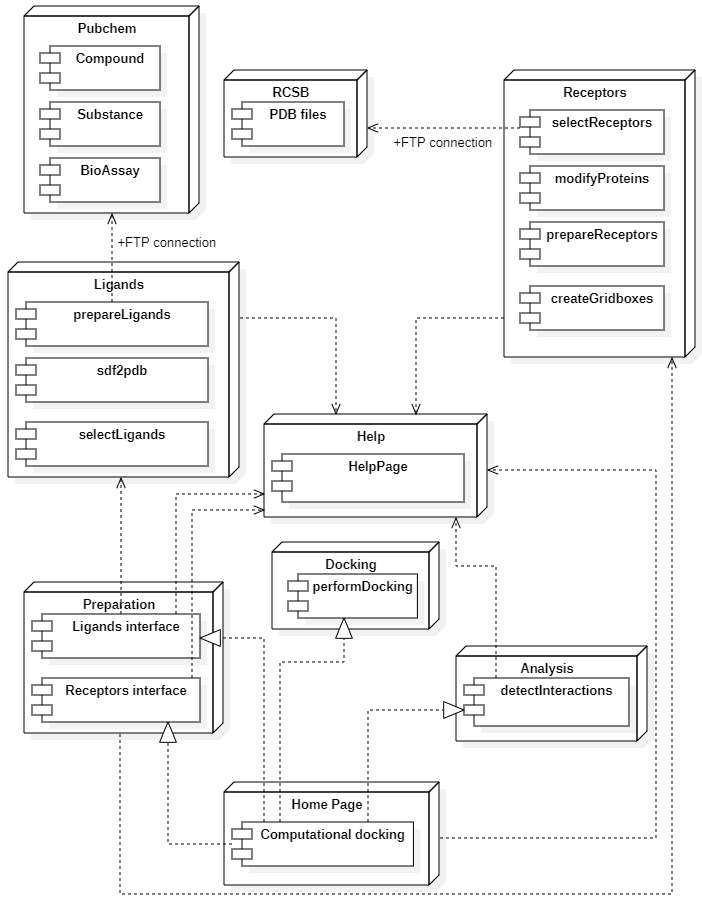
\includegraphics[scale=0.9]{immagini/capitolo1/UML.png}
    \caption{Diagramma implementativo del software}
    \label{fig:UML}
\end{figure}